\documentclass[12pt,a4paper,UTF8]{article}
% \usepackage{ctex} % Chinese support
\usepackage{graphicx} % Insert images
\usepackage{listings} % Print source code
\usepackage{color} % Color support
\usepackage{booktabs} % Professional table support
\usepackage{pdflscape} % Landscape pages support in PDF
\usepackage{hyperref} % Hypertext links support for cross-referencing

% Customize hyperref format (it's set to no special format here)
\hypersetup{hidelinks}

% Declare directories to search for graphics files for graphicx
\graphicspath{{figures/}{logo/}}

% Define source code style for listings
\lstdefinestyle{python}{
  language=Python,
  basicstyle=\ttfamily\footnotesize,
  keywordstyle=\bfseries\color[rgb]{0, 0, 1},
  identifierstyle=\color[rgb]{0.5, 0.3, 0.1},
  stringstyle=\color[rgb]{0.6, 0.1, 0.1},
  commentstyle=\itshape\color[rgb]{0.05, 0.5, 0.05},
  backgroundcolor=\color[gray]{0.95},
  numbers=left,
  numbersep=5pt,
  numberstyle=\color[gray]{0.6},
  breaklines=true
}

% Define new command for title page
\newcommand{\reporttitle}[2]{
  \LARGE\textsf{#1}\quad\underline{\makebox[12em]{#2}}
}
\newcommand{\reportinfo}[2]{
  \large\makebox[4em]{\textsf{#1}}\quad\underline{\makebox[18em]{#2}}
}

% The document begins here
\begin{document}
\begin{titlepage}
  \centering
  \vspace*{\fill}
  
\includegraphics[height=144pt]{nju-logo}\\[48pt]
  {\huge\textsf{Lab Report}}\\[48pt]
  \reporttitle{Lab Name}{Switch}\\[72pt]

  \reportinfo{Course}{Computer Network}\\[8pt]
  \reportinfo{Major}{Computer Science and Technology}\\[8pt]
  \reportinfo{Id}{191220129}\\[8pt]
  \reportinfo{Name}{Shangyu.Xing}\\[8pt]
  \reportinfo{Email}{191220129@smail.nju.edu.cn}\\[8pt]
  \reportinfo{Date}{2021.03}\\
  \vspace*{\fill}
\end{titlepage}

\tableofcontents
\newpage

\section{Objective}
\begin{itemize}
	\item Learn core functionalities of an Ethernet learning switch;
	\item learn to implement hardware logic using the Switchyard framework;
	\item learn to capture network package using wireshark.
\end{itemize}

\section{Requirements}
This lab requires to implement the core functionalities of an Ethernet learning switch. Specific tasks are as follows.
\begin{itemize}
	\item Implement a basic learning switch;
	\item implement a learning switch with timeout mechanism;
	\item implement a learning switch with least recently used mechanism;
	\item implement a learning switch with least traffic volume mechanism;
\end{itemize}

\section{Procedure}
In this section, I will explain how I implement the switch with different mechanism in detail. \\
Although the three mechanisms resemble little with one another, their behavior as a switch remains consistent. The general procedure of a switch processing an incoming packet is listed as follows:
\begin{enumerate}
	\item Do some update to its forwarding table according to the source address and the specific mechanism;
	\item Look its forwarding table for an entry with the destination address;
	\begin{itemize}
		\item if found, do some update to its forwarding table according to the specific mechanism, and then forward the packet to the destination address;
		\item if not found, flood the packet out all ports except the incoming one.
	\end{itemize}
\end{enumerate}
According to the features, we can do some high-level abstraction. I established a python class called ForwardTable to encapsulate the behavior of different mechanisms. The class template is here.
\lstinputlisting[style=python]{1.py}

After implementing the above class for every mechanism, we are free from the worry of the different mechanisms. All we have to is to write a uniform main function regardless of the specific mechanism to implement the switch functionality.
\\ The uniform main function is as follows.
\lstinputlisting[style=python]{2.py}

\subsection{Basic Switch}
There is no status information to maintain, so the implementation of the ForwardTable class is very simple.
\lstinputlisting[style=python]{3.py}

\subsection{Timeout}
In this part we need to maintain a status information: timestamp. Timestamp is updated when a new packet arrived. If the timestamp of an entry is older than timeout value, the entry is considered invalid, and query of it should return None.
\lstinputlisting[style=python]{4.py}

\subsection{Least Recently Used}
The status information here is age. Age of all entries is incremented by 1 whenever a new packet arrives. If the number of entries is larger than max\_size, the oldest entry is removed.
\lstinputlisting[style=python]{5.py}

\subsection{Least Traffic Volume}
Here we need to record traffic volume for each entry. Traffic of the corresponding entry is increased by 1 when a new packet arrives. If the number of entries is larger than max\_size, the entry with least traffic volume is removed.
\lstinputlisting[style=python]{6.py}

\section{Result}
\subsection{Basic Switch}
The procedure of the switch's forwarding is as follows:
\begin{enumerate}
	\item The client broadcast arp packet, and the switch learned that the client is related to a certain interface;
	\item the server reply arp packet to the client, and the switch learned another entry;
	\item the client send echo request to the server, and the switch forward the packet according to its forwarding table;
	\item the server broadcast arp packet;
	\item the client reply arp packet, and the switch forward the packet according to its forwarding table;
	\item the server send echo reply to the client, and the switch forward the packet according to its forwarding table;
	\item repeat procedure 3, 6.
\end{enumerate}
As a result, wireshark can capture echo packet in server1 but cannot capture echo packet in server2.

\subsection{Timeout}
Switchyard test result:
\begin{figure}[htbp]
	\centering
	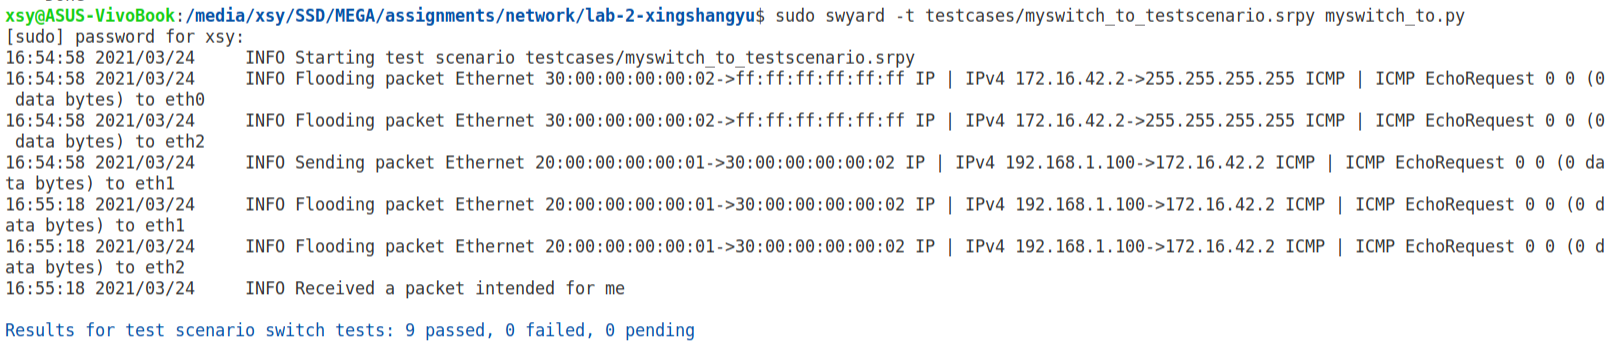
\includegraphics[width=\textwidth]{to_test}
	\caption{Timeout test result}
\end{figure}
\newpage
Mininet test(using command: \\ client ping -c 1 server1 \\ (after 5s) repeat \\ (after 15s) repeat \\ )
\begin{figure}[htbp]
	\centering
	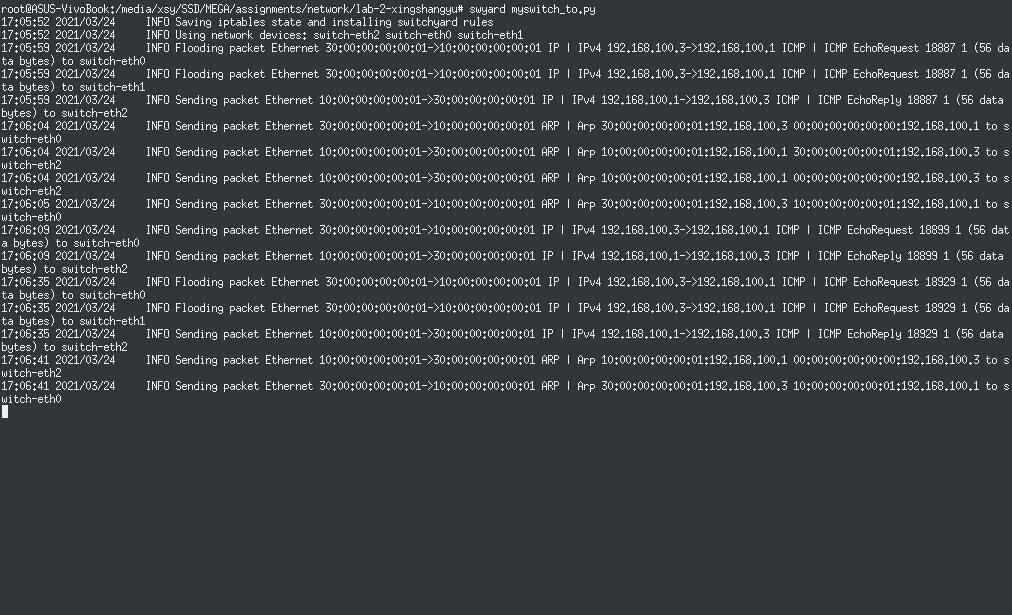
\includegraphics[width=\textwidth]{to_mininet}
	\caption{Switch log}
\end{figure}
\\ As can be seen in the picture above, the entries in forwarding table did not timeout in 5s but timeout after 15s.

\subsection{Least Recently Used}
Switchyard test result:
\begin{figure}[htbp]
	\centering
	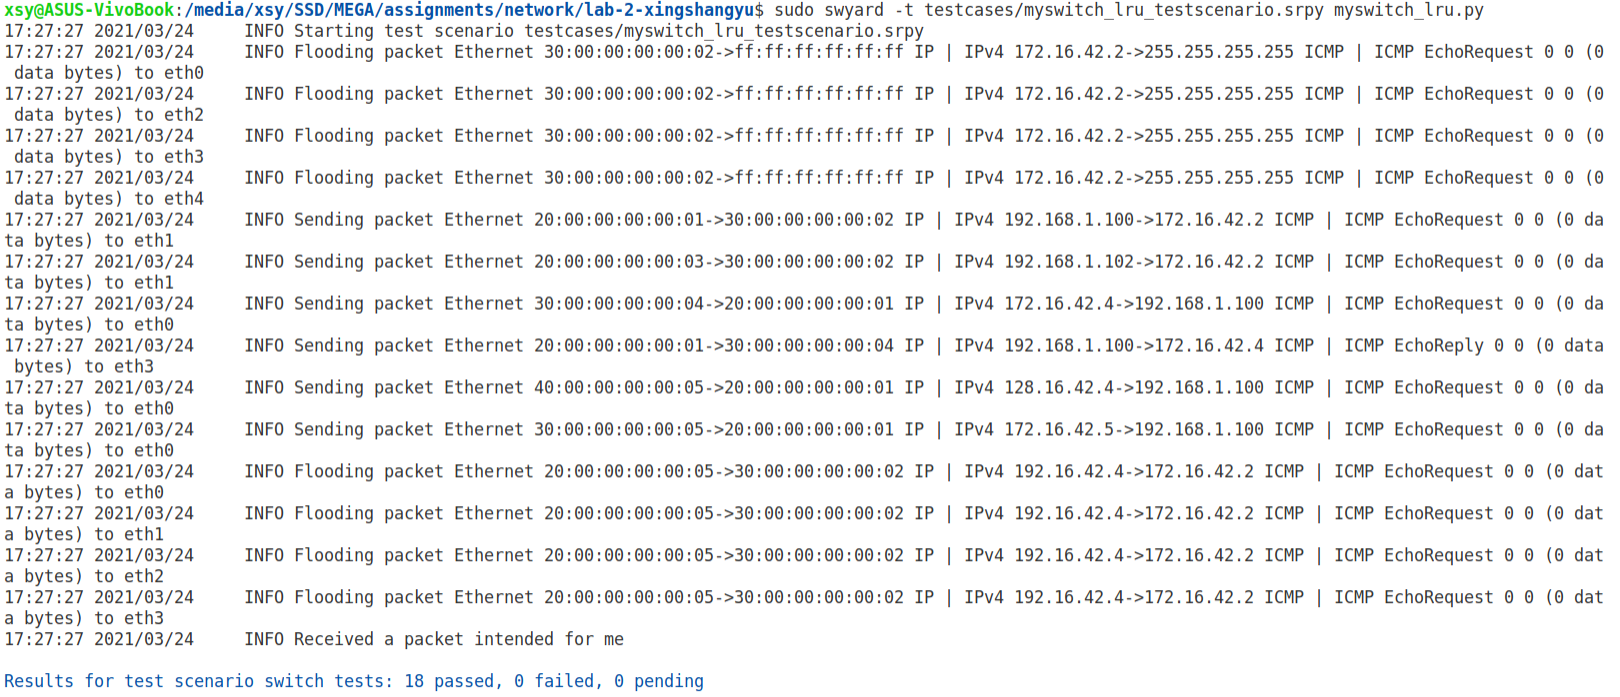
\includegraphics[width=\textwidth]{lru_test}
	\caption{Least recently used test result}
\end{figure}
\newpage
Mininet test(setting table capacity to 2, using command: \\ client ping -c 1 server1; \\ client ping -c 1 server2; \\ client ping -c 1 server1 \\ )
\begin{figure}[htbp]
	\centering
	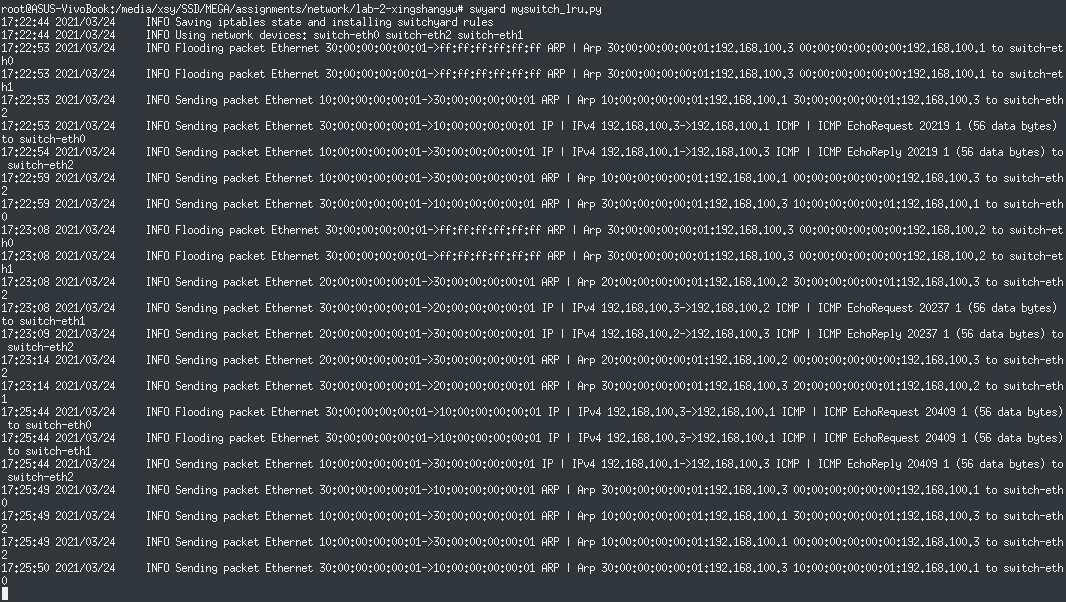
\includegraphics[width=\textwidth]{lru_mininet}
	\caption{Switch log}
\end{figure}
\newpage
As can be seen in the picture above, the least recently used entry(10:00:00:00:00:01) in forwarding table is removed when the second command is executed.

\subsection{Least Traffic Volume}
Switchyard test result:
\begin{figure}[htbp]
	\centering
	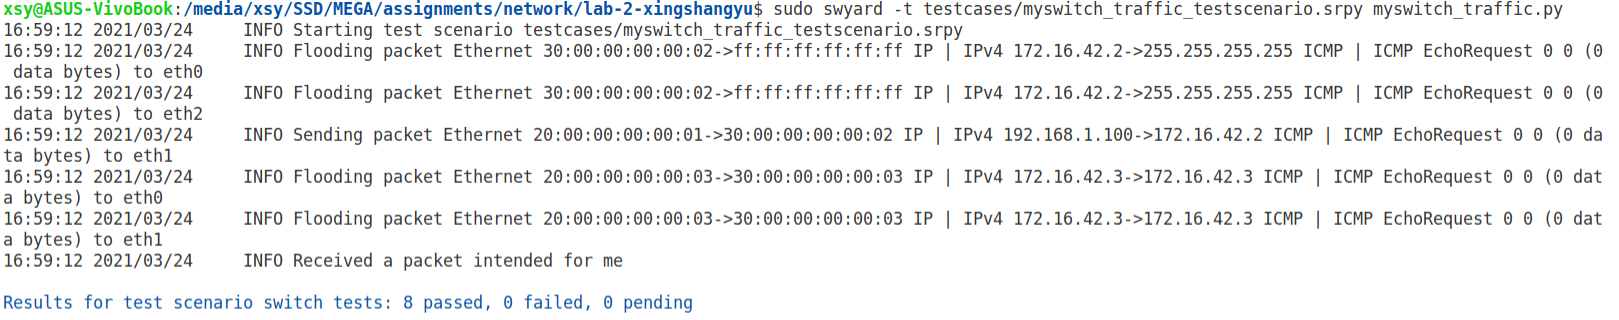
\includegraphics[width=\textwidth]{traffic_test}
	\caption{Least Traffic Volume test result}
\end{figure}
\\ Mininet test(setting table capacity to 2, using command: \\ client ping -c 1 server1; \\ client ping -c 1 server2; \\ client ping -c 1 server1 \\ )
\begin{figure}[htbp]
	\centering
	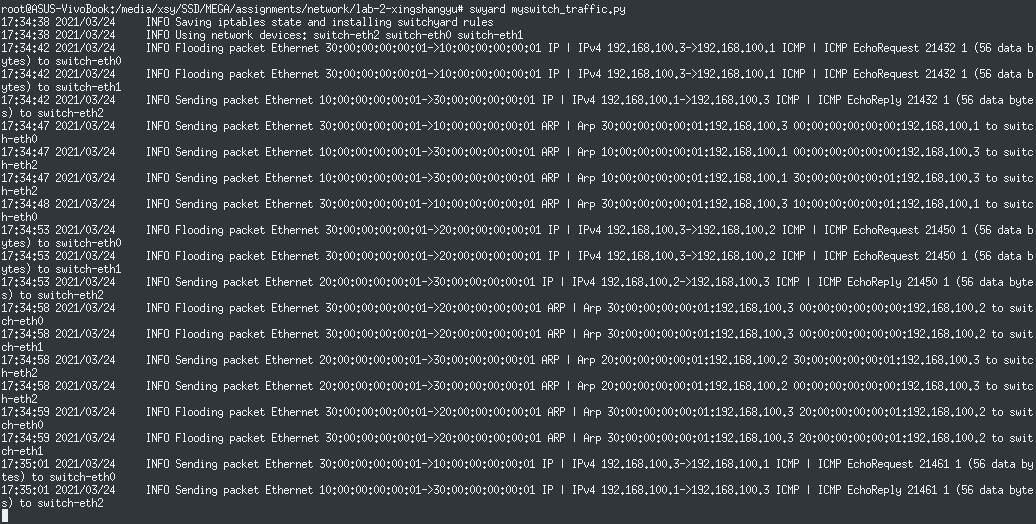
\includegraphics[width=\textwidth]{traffic_mininet}
	\caption{Switch log}
\end{figure}
\newpage
As can be seen in the picture above, the entry woth least traffic volume(20:00:00:00:00:01) in forwarding table is removed when the second command is executed.

\section{Summary}
\begin{itemize}
	\item Knowing how to use tools effectively will greatly enhance working efficiency;
	\item English reading and writing skills are important.
\end{itemize}

\end{document}